\begin{slide}
\pagestyle{headings}
\sf
\header{Generalisation to any one-parameter fit}

\Large 
%For any fit with one single parameter $a$:\\
{\em Taylor expansion} of $\chi^2$ around estimated value $\hat{a}$:
\[ 
\chi^2 = \chi^2(\hat{a}) + \frac{d\chi^2}{da}_{|a=\hat{a}} 
\cdot (a - \hat{a}) + \frac{1}{2}\, 
\frac{d^2\chi^2}{da^2}_{|a=\hat{a}}
\cdot (a - \hat{a})^2 + ...
\]
\[ = \chi^2(\hat{a}) + H \cdot (a - \hat{a})^2 \quad
\mbox{with} \quad H = \frac{1}{2}\,\frac{d^2\chi^2}{da^2}_{|a=\hat{a}}
\quad \mbox{Hesse matrix}
\]
Thus the {\em inverse probability density} is 
\[
 p(a|\hat{a}) \sim e^{-\frac{\chi^2(\hat{a})}{2}}
 \cdot 
e^{-\frac{1}{2}\, H \cdot (\hat{a}-a)^2) } 
\]
$\rightarrow$ Gaussian distribution around $\hat{a}$ with
width $\sigma = H^{-1/2}$

\end{slide}
\begin{slide}
\pagestyle{headings}
\sf
\header{Generalisation to any one-parameter fit}
\Large 


\[ \chi^2(a) = \chi^2(\hat{a}) + 
\frac{(a-\hat{a})^2}{\sigma^2} \]
\[ \rightarrow \quad \chi^2(a \pm 1 \sigma) = \chi^2(\hat{a}) + 1 
= \chi^2_{min} + 1 
\]
%$\rightarrow$ Read error directly from $\chi^2$ curve
%
%
\begin{figure}[h]
\unitlength1cm
  \begin{picture}(8,7.5)
    \put(0.,0.){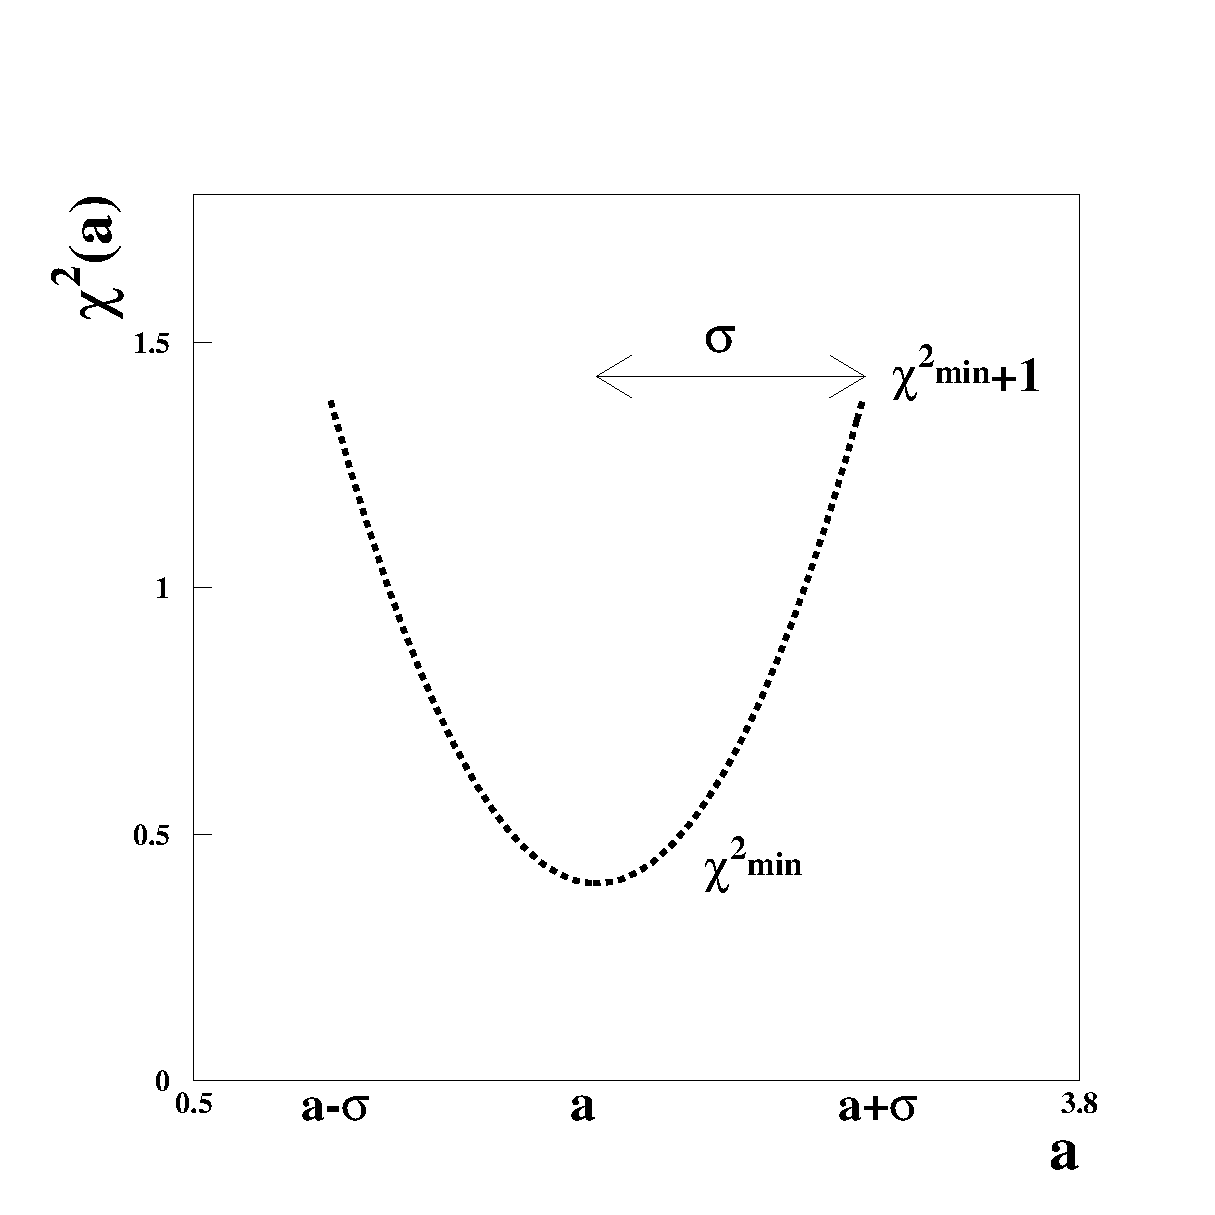
\epsfig{file=feynman/chisqp2.epsi,width=8.cm}}
     \put(8.,5.5){
\begin{minipage}[t]{7cm} 
$\rightarrow$ Read error directly\\ 
from $\chi^2$ curve
\end{minipage}
}
%    \put(8.,5.){\LARGE $\chi^2(\hat{a}+\sigma_{\hat{a}}) = 1$}
\end{picture}
\end{figure}
\vfill
\end{slide}
